
\title{Building Orbiter Sample Programs}

\documentclass[a4paper]{article}
\usepackage{times}
\usepackage{cite}
\usepackage{hyperref}
\usepackage{geometry}
\usepackage{graphicx}

\geometry{
 a4paper,
 total={160mm,240mm},
 left=30mm,
 top=30mm,
 }

\begin{document}
\maketitle

\section{Getting everything ready}
There are probably many ways to build the sample programs from a CMake scripts but I'll give instructions to a method I am most familiar with.
First you need to download CMake \href{https://cmake.org/download/}{https://cmake.org/download/} and install it. After installation you should be seeing following icon on your Desktop. Click it. 

\begin{center}
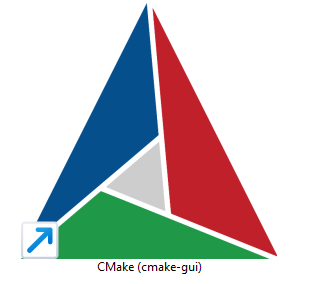
\includegraphics[width=0.15\linewidth]{assets/cmakeicon.png}
\end{center}

After launching the CMake you will see CMake's VS-genarator interface to pop-up.

\begin{center}
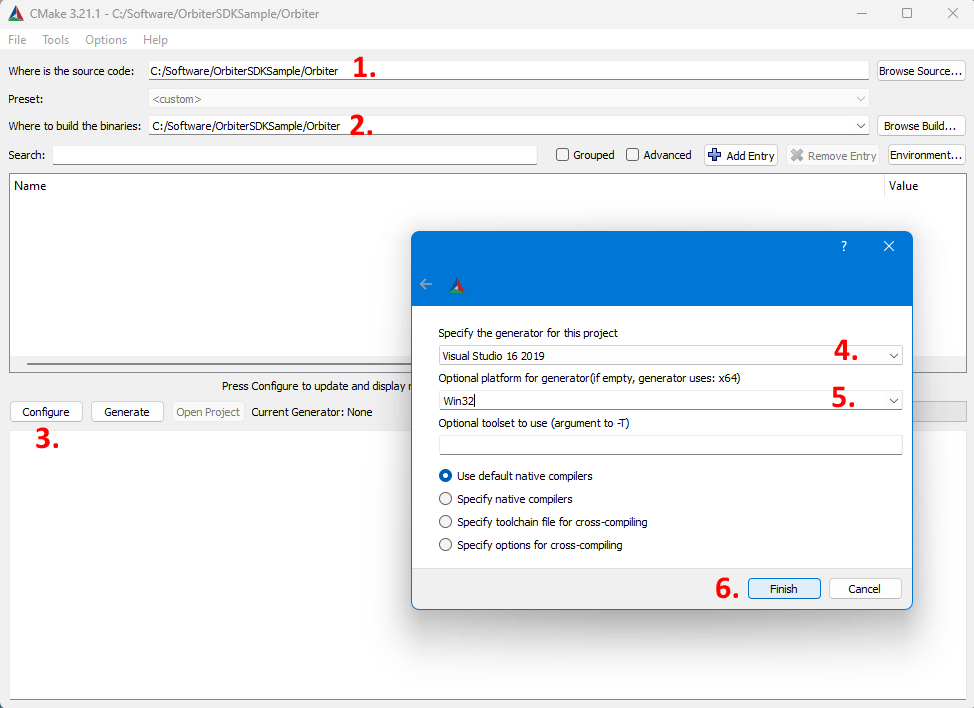
\includegraphics[width=1.0\linewidth]{assets/vsgen1.png}
\end{center}
\newpage

\begin{itemize}
\item To position 1. setup path to Orbiter's \textit{root} folder
\item To position 2. also setup path to Orbiter \textit{root}.
\item Click "\textbf{Configure}" and a new dialog screen will pop-up.
\item Select your "Visual Studio" version.
\item Select "\textbf{Win32}" architecture (platform as indicated by the text) that will compile 32-bit (x86) binaries. Orbiter2024 is x86 program. Future versions may use x64 architecture.
\item Click "\textbf{Finish}" when done.
\item Finally press "\textbf{Generate}". As a result Visual Studio solution and project files will be placed in Orbiter \textit{root} and \textit{Orbitersdk/samples} folder.
\end{itemize}

\vspace{1cm}

\begin{center}
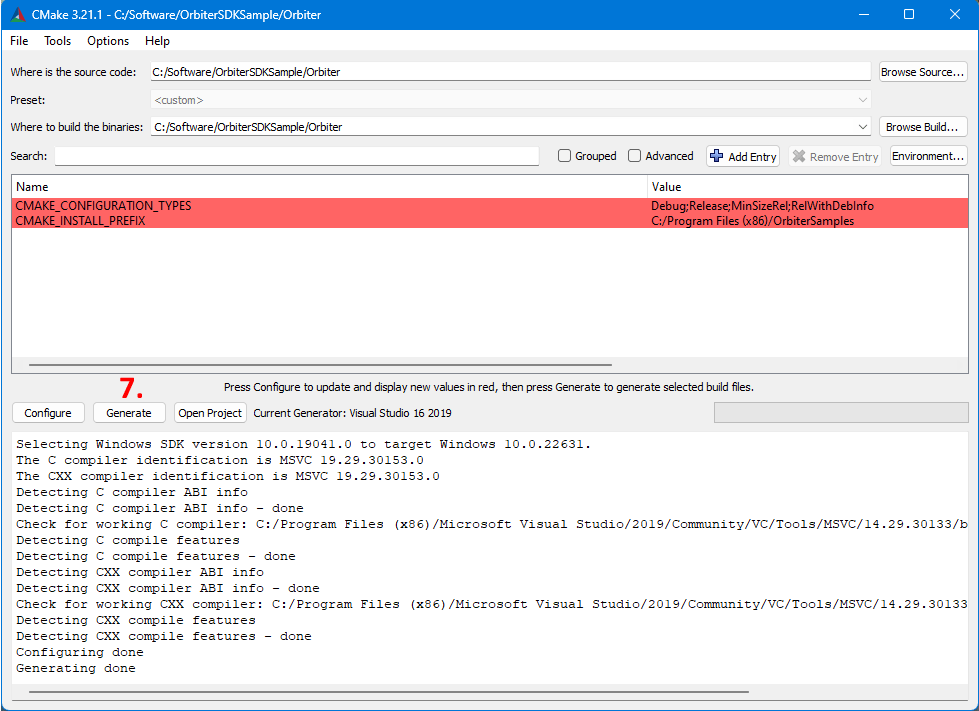
\includegraphics[width=1.0\linewidth]{assets/vsgen2.png}
\end{center}

\vspace{1cm}

Current CMake configuration scripts are using your Orbiter's installation folder as build directory. This removes a need of separate install procedure but it will add some pollution to Orbiter \textit{root} and much more in \textit{samples} folder. When done go to Orbiter \textit{root} and launch "`\textbf{OrbiterSamples.sln}" which should open Visual Studio program. Don't worry about the red lines shown in the application. The "\textit{install prefix}" would be important if an installation procedure would be in use but it's not.

\begin{center}
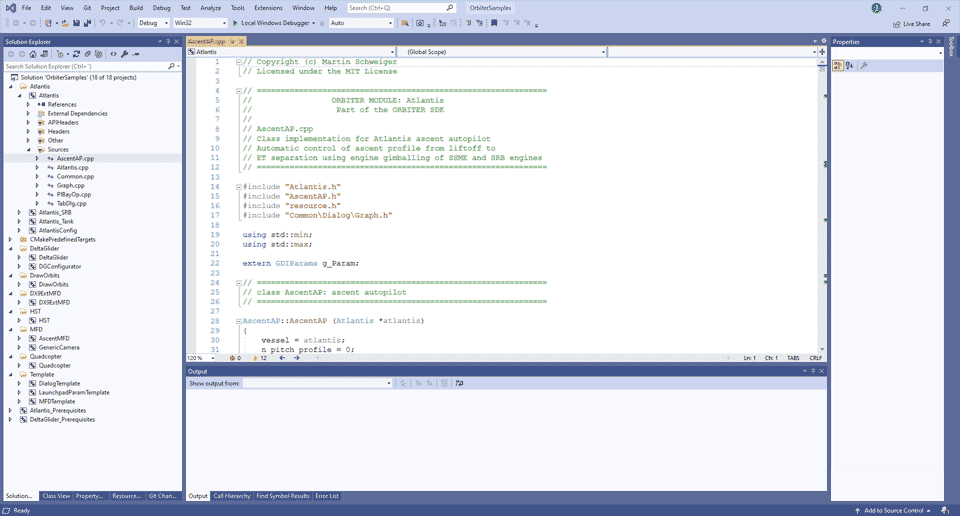
\includegraphics[width=1.0\linewidth]{assets/vs.png}
\end{center}

\end{document}
